\chapter{个人研究进展}
\label{chap:personal_research}

在对混合专家模型（Mixture-of-Experts, MoE）架构与训练策略进行广泛而深入的调研基础上，我们识别出负载均衡（Load Balancing）是制约其性能和训练稳定性的核心挑战之一。经典的负载均衡策略，如第\ref{sec:aux_loss}节所述，通常依赖于一个辅助损失函数（Auxiliary Loss）来鼓励路由器（Router）将计算负载均匀地分配给所有专家（Experts）。然而，这种方法引入了一个固有的权衡难题：一个较弱的辅助损失可能无法有效解决负载不均衡问题，甚至导致部分专家训练不足，发生“路由坍缩”（Routing Collapse）现象；而一个较强的辅助损失则会产生不容忽视的干扰梯度（Interference Gradients），这些梯度与模型主要的语言建模目标相冲突，从而损害模型的最终性能。

为了打破这种“性能-均衡”的困境，我们进行了深入的探索，并提出了一种创新的、无需辅助损失的负载均衡策略，我们将其命名为\textbf{无辅助损失均衡（Auxiliary-Loss-Free Balancing）} \cite{Wang2024AuxiliaryLossFreeLB}。本章将详细阐述该策略的核心思想、算法设计、实验验证与分析。这项工作旨在为大规模混合专家模型的训练提供一种更高效、更稳定的负载均衡解决方案。

\section{动机：辅助损失的困境}
\label{sec:motivation_dilemma}

如第\ref{sec:aux_loss}节所述，现有的混合专家模型广泛采用辅助损失函数来引导负载均衡。该损失函数通常定义为：
\begin{equation}
    L_{\text{Balance}} = \alpha \cdot N \sum_{i=1}^{N} (f_i \cdot P_i)
\end{equation}
其中，$\alpha$ 是控制均衡强度的超参数，$N$ 是专家总数，$f_i$ 是路由到第 $i$ 个专家的词元（Token）比例，$P_i$ 是第 $i$ 个专家获得的平均门控权重（Gating Weights）。

这个辅助损失项虽然能够促进负载均衡，但也作为一个正则化项，引入了与主任务（如语言建模）无关的梯度。如图\ref{fig:dilemma_balance_performance}所示，超参数 $\alpha$ 的选择直接导致了模型性能和负载均衡之间的两难局面。当 $\alpha$ 值较小（例如 $10^{-4}$）时，虽然模型性能较好，但负载均衡效果差，容易导致路由坍缩。相反，当 $\alpha$ 值较大（例如 $10^{-2}$）时，负载均衡（以第\ref{sec:ep_and_lb}节中提及的最大负载违规率衡量）得到保证，但模型的性能（以困惑度 Perplexity 衡量）会显著下降。

\begin{figure}[h]
    \centering
    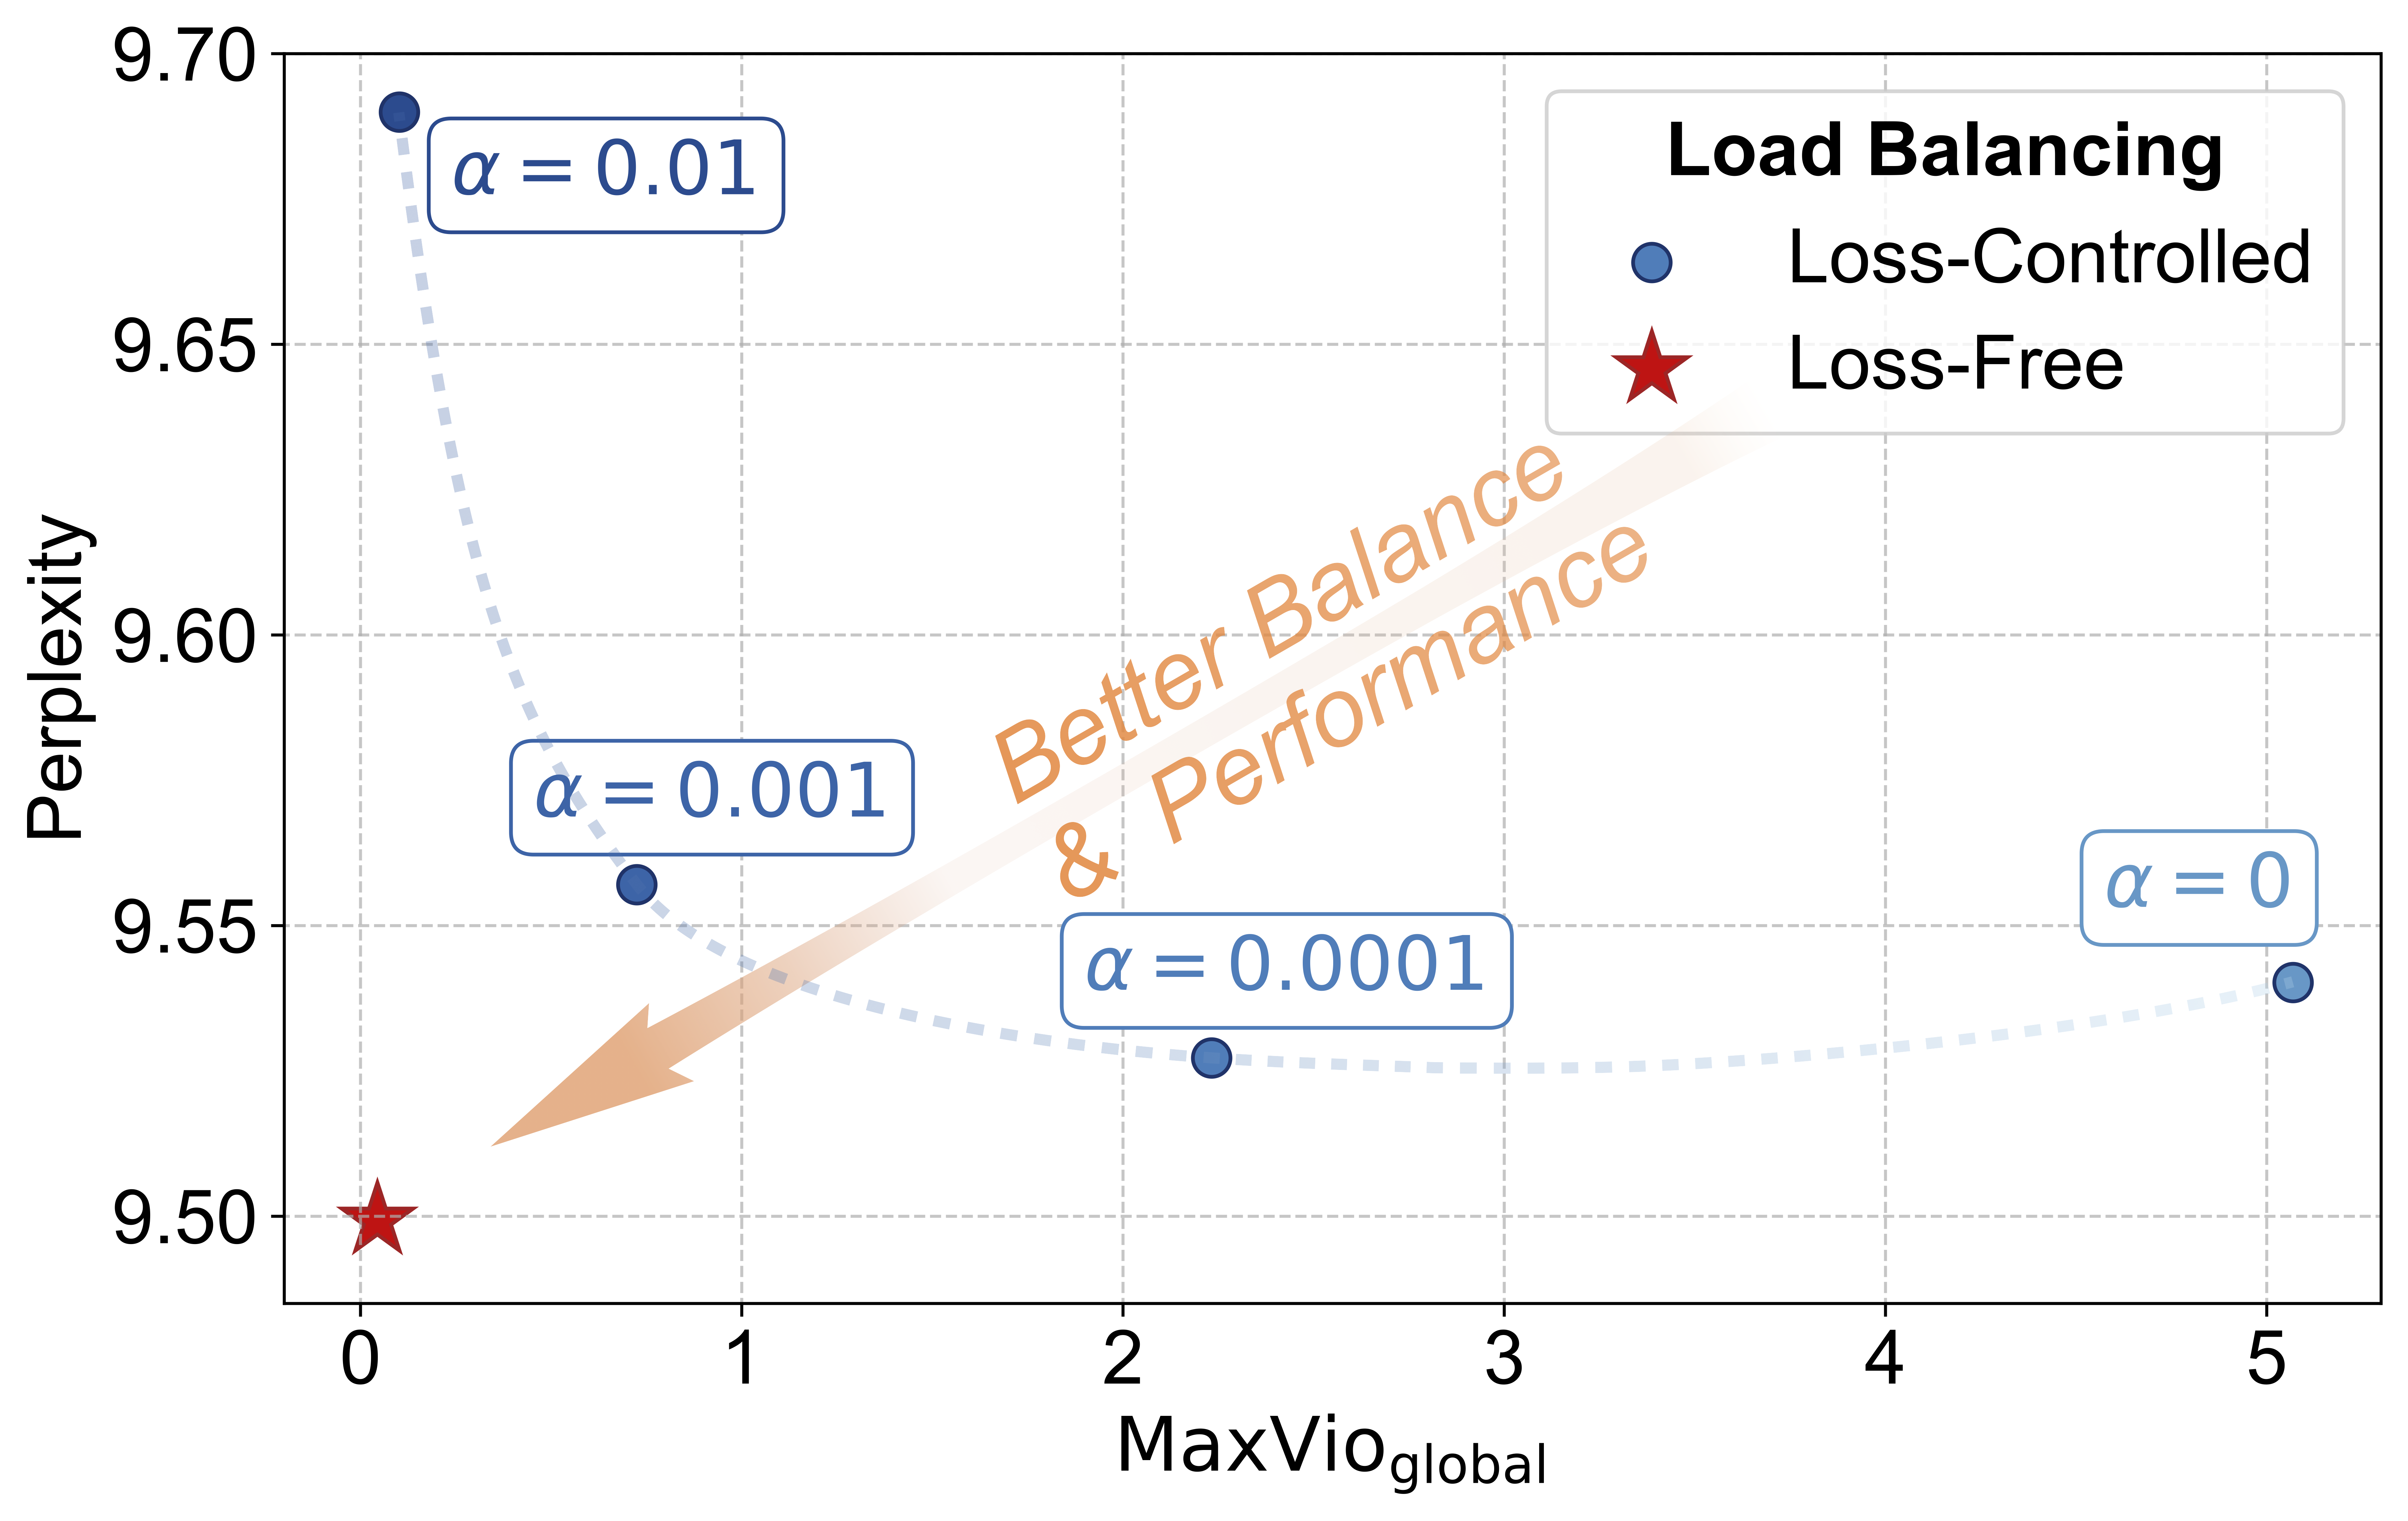
\includegraphics[width=0.8\textwidth]{figures/my_paper/balance_mv_perplexity_new_new.png}
    \caption{辅助损失控制下的负载均衡与模型性能困境。我们的无辅助损失均衡方法（红色星号）成功地打破了这一困境，同时实现了更优的性能和更好的负载均衡。}
    \label{fig:dilemma_balance_performance}
\end{figure}

这种固有的冲突表明，基于辅助损失的负载均衡策略可能并非最优解。理想的策略应该能够在不干扰主任务训练的前提下，直接且有效地控制专家负载。正是基于这一动机，我们设计了无辅助损失均衡策略。

% unfinished

\section{无辅助损失均衡（Auxiliary-Loss-Free Balancing）策略}
\label{sec:loss_free_balancing}

无辅助损失均衡策略的核心思想是：\textbf{不通过损失函数和梯度反向传播来间接“惩罚”不均衡，而是通过直接调整路由过程中的专家得分来实现主动“引导”均衡}。具体而言，我们在路由器计算出每个专家的原始路由得分（Routing Scores）之后，但在进行 Top-K 选择之前，为每个专家引入一个可动态调整的偏置项（Bias Term）。

\subsection{算法原理}

在每个训练步骤中，无辅助损失均衡策略包含两个核心环节：带偏置的专家选择和偏置项的动态更新。其工作流程如图 \ref{fig:lfb_workflow} 所示。

\begin{figure}[h]
    \centering
    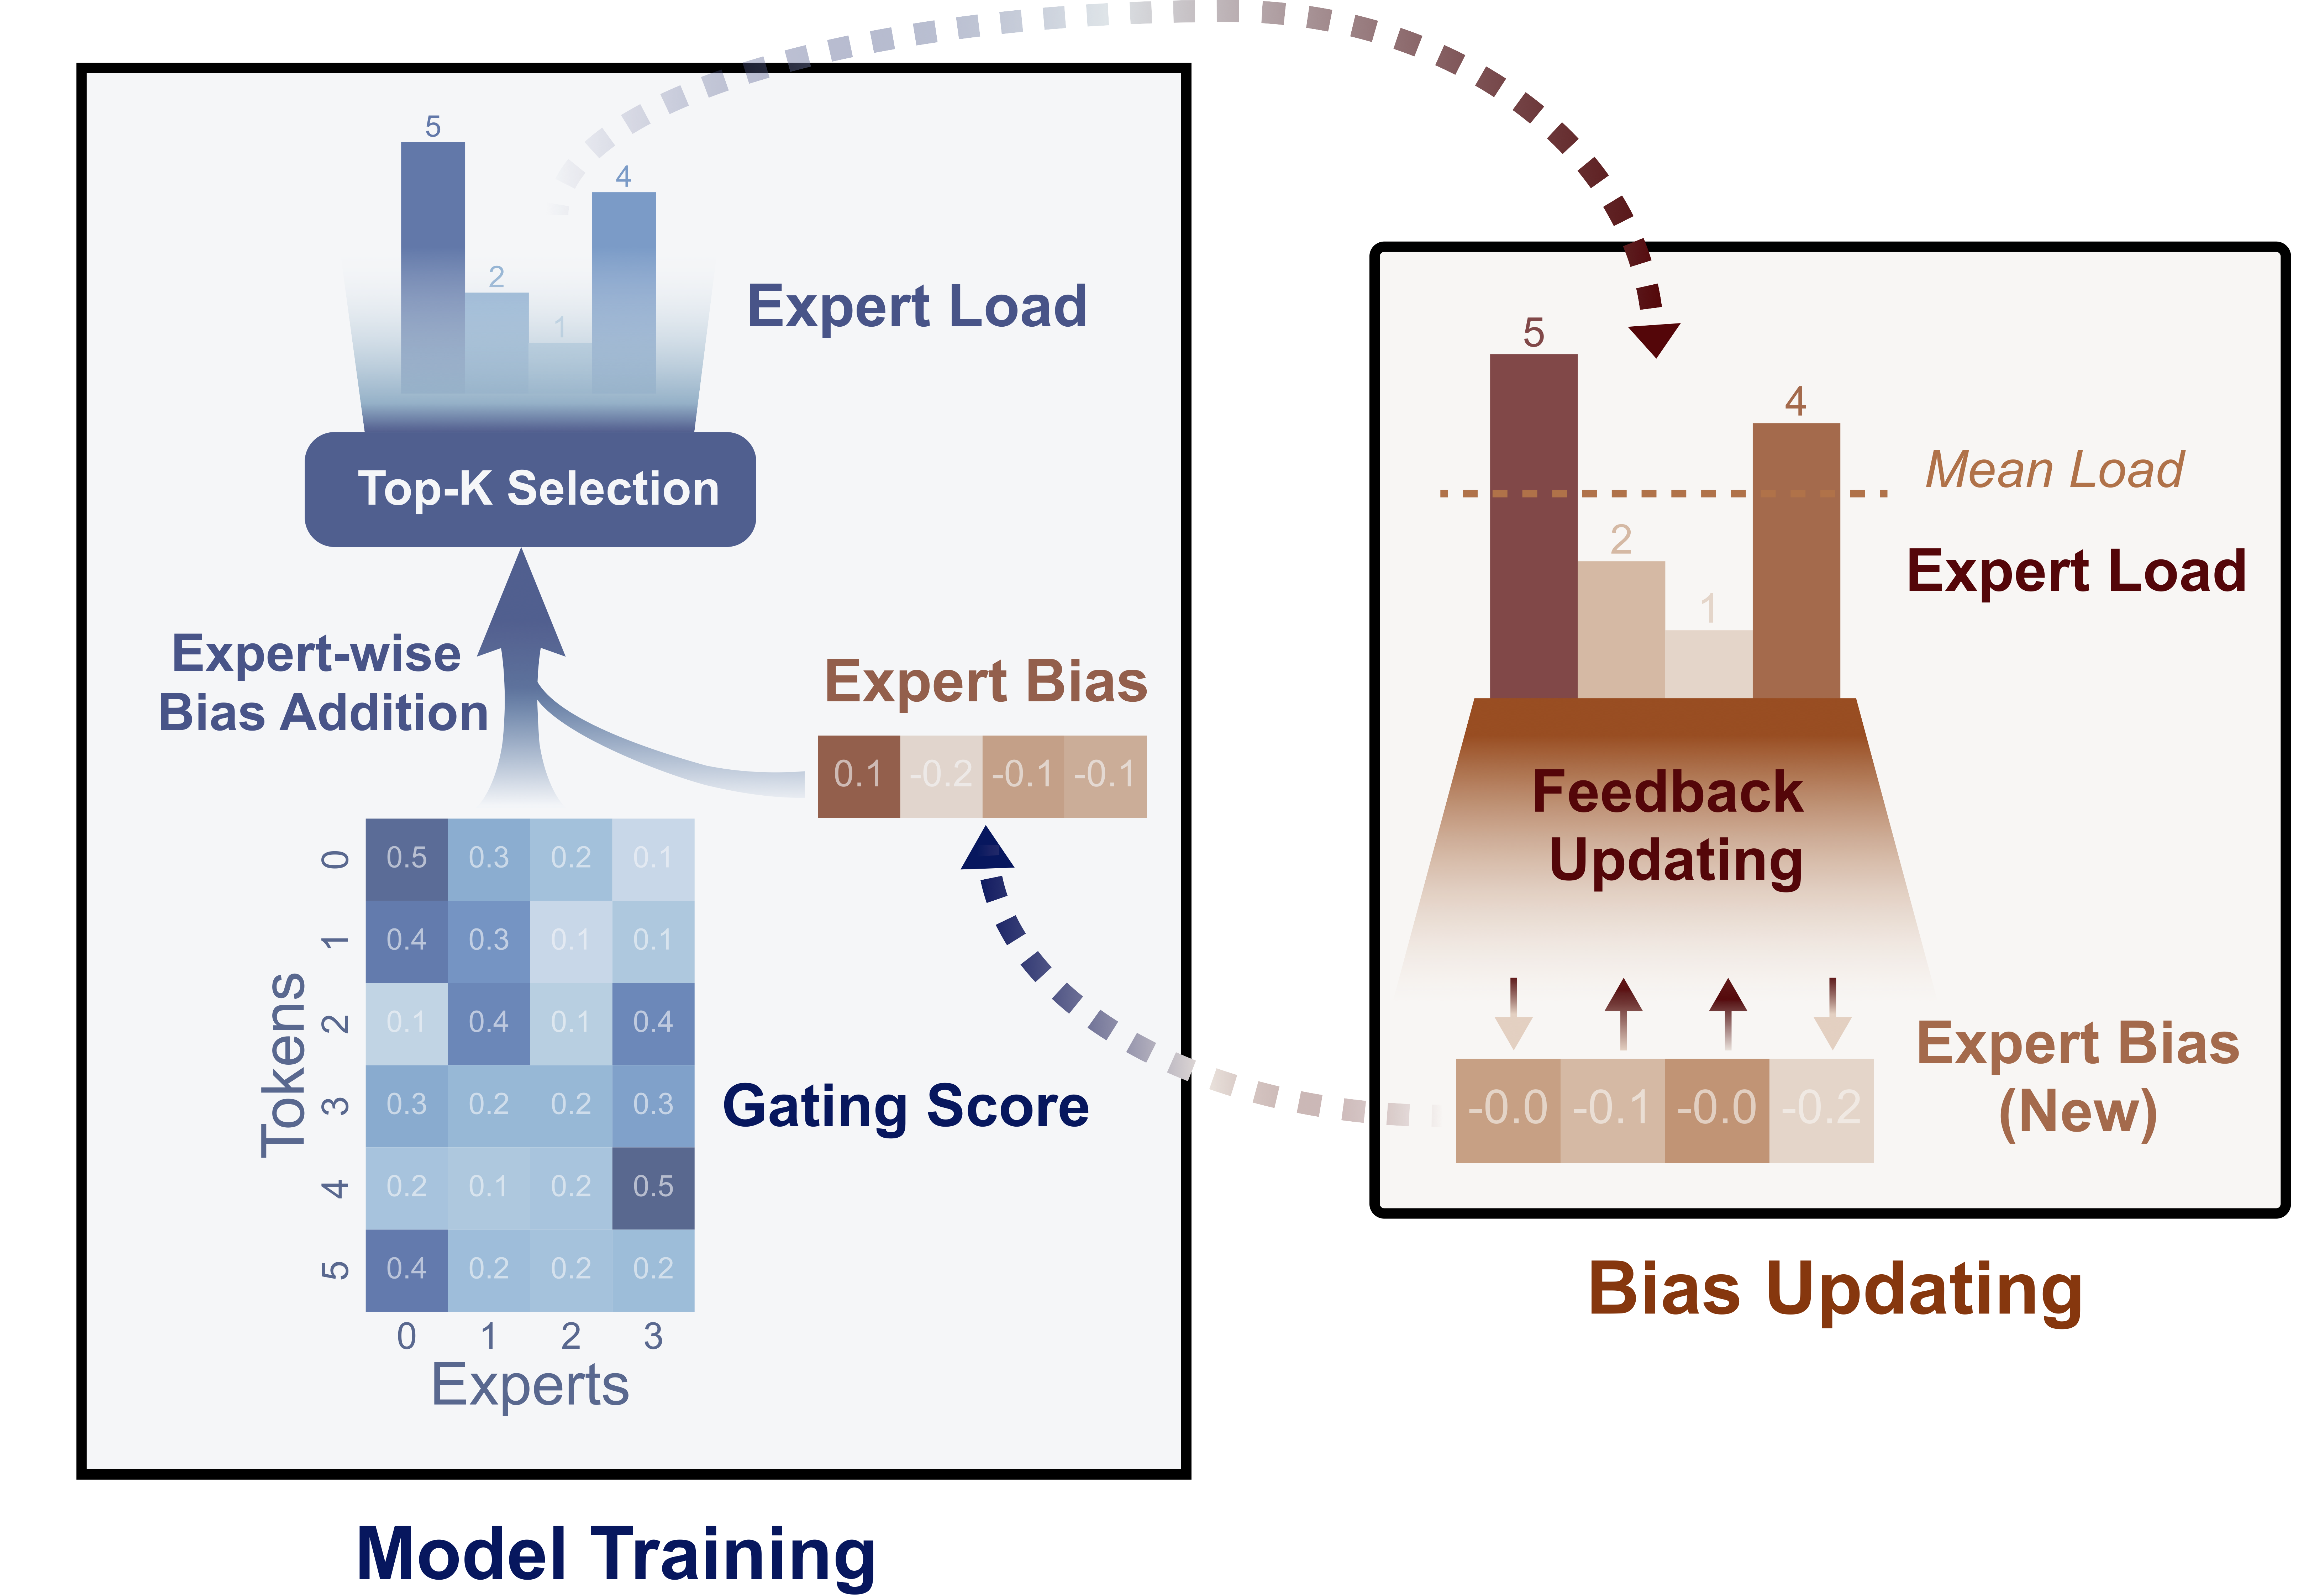
\includegraphics[width=0.9\textwidth]{figures/my_paper/figure_815.png}
    \caption{无辅助损失均衡策略的工作流程示意图。在每个训练步骤中，模型首先根据带有偏置的门控分数选择专家，然后在该步骤结束后，根据最近的专家负载情况反馈更新偏置项。}
    \label{fig:lfb_workflow}
\end{figure}

\paragraph{带偏置的专家选择}
对于一个输入词元 $x_t$，路由器首先计算出其对于所有 $N$ 个专家的原始路由得分 $s_{i,t}$。在经典的 Top-K 路由中，模型会直接从 $\{s_{j,t}\}_{j=1}^N$ 中选择得分最高的 K 个专家。而在我们的无辅助损失均衡策略中，我们会先为每个专家的得分加上一个对应的偏置项 $b_i$，然后再进行 Top-K 选择。因此，门控值 $g_{i,t}$ 的计算方式变为：
\begin{equation}
\label{eq:bias_gate}
    g_{i,t} = 
    \begin{cases}
        s_{i,t}, & \text{若 } s_{i,t} + b_i \in \text{TopK}(\{s_{j,t} + b_j | 1 \le j \le N\}, K) \\
        0, & \text{其他情况}
    \end{cases}
\end{equation}
至关重要的是，这个偏置项 $b_i$ \textbf{仅用于影响 Top-K 的选择过程}，它本身并不会被加到最终用于加权专家输出的门控值 $g_{i,t}$ 上，因此不会引入任何干扰梯度。

\paragraph{偏置项的动态更新}
偏置项 $\{b_i\}_{i=1}^N$ 的设计目标是动态地反映每个专家的负载情况。其更新遵循一个简单的原则：对于近期负载较重（被分配词元过多）的专家，降低其偏置值，从而在后续的路由选择中降低其被选中的概率；反之，对于近期负载较轻的专家，则提高其偏置值。

在每个训练批次（batch）结束后，我们首先统计该批次中每个专家 $i$ 被分配到的词元数量 $c_i$。然后，我们计算所有专家的平均负载 $\bar{c}$。基于此，我们可以得到每个专家的负载违规误差（Load Violation Error）$e_i = c_i - \bar{c}$。偏置项的更新算法如下：

% \begin{algorithm}[H]
% \caption{训练过程中调整各专家偏置 $b_i$}
% \begin{algorithmic}
% \REQUIRE MoE 模型 $\theta$，训练批次迭代器 $\mathcal{B}$，偏置更新率 $u$。
% \STATE 初始化所有专家的偏置 $b_i = 0$。
% \FOR{每个批次 $\{(x_k, y_k)\}_k \in \mathcal{B}$}
%     \STATE 2. 根据公式 (5.2) 计算门控得分，在批次数据上训练 MoE 模型 $\theta$。
%     \STATE 3. 统计每个专家被分配的词元数 $c_i$，并计算平均负载 $\bar{c}$。
%     \STATE 4. 计算负载违规误差 $e_i = c_i - \bar{c}$。
%     \STATE 5. 更新偏置：$b_i \leftarrow b_i - u \cdot \text{sign}(e_i)$。
% \ENDFOR
% \ENSURE 训练好的模型 $\theta$ 及对应的偏置 $b_i$。
% \end{algorithmic}
% \end{algorithm}
\begin{algorithm}[t]
\SetAlgoLined
% \KwResult{Result of the algorithm}
\KwIn{MoE 模型 $\theta$，训练批次迭代器 $\mathcal{B}$，偏置更新率 $u$。}
% \KwOut{Here, provide the expected output/results of your algorithm}
1. 初始化所有专家的偏置 $b_i = 0$\;
\For{每个批次 $\{(x_k, y_k)\}_k \in \mathcal{B}$}{
    2. 根据公式\ref{eq:bias_gate}计算门控得分，在本批次数据上训练 MoE 模型 $\theta$\;
    3. 统计每个专家被分配的词元数 $c_i$，并计算平均负载 $\bar{c}$\;
    4. 计算负载违规误差 $e_i = c_i - \bar{c}$\;
    4. 更新偏置：$b_i \leftarrow b_i - u \cdot \text{sign}(e_i)$\;
}
\KwOut{trained model $\theta$, corresponding bias $\mathbf b_i$}
\caption{训练过程中调整各专家偏置 $b_i$}
\label{algo:PID_gate}
\end{algorithm}


值得注意的是，在这里，偏置的更新是基于历史批次的负载信息，这确保了语言建模的因果约束（Causal Constraint）不被破坏，避免了未来词元信息（Future Token Leakage）的泄露。

\subsection{方法优势}
\label{sec:theoretical_advantages}
相比于传统的辅助损失方法和其他主流的负载均衡策略（如专家选择路由 Expert Choice），无辅助损失均衡策略具备多项优势，如表 \ref{tab:method_comparison} 所示。

\begin{table}[htbp]
    \centering
    \caption{不同负载均衡方法的特性比较。绿色表示优良特性，红色表示不良特性。}
    \begin{tabular}{l|ccc}
        \toprule
        \textbf{负载均衡方法} & \textbf{均衡的专家负载} & \textbf{干扰梯度} & \textbf{未来词元泄露} \\
        \midrule
        辅助损失（强） & \textcolor{green}{balanced} & \textcolor{red}{strong} & \textcolor{green}{no leakage} \\
        辅助损失（弱） & \textcolor{red}{imbalanced} & \textcolor{red}{weak} & \textcolor{green}{no leakage} \\
        专家选择（EC） & \textcolor{green}{balanced} & \textcolor{green}{none} & \textcolor{red}{with leakage} \\
        \textbf{无辅助损失均衡（我们的）} & \textcolor{green}{balanced} & \textcolor{green}{none} & \textcolor{green}{no leakage} \\
        \bottomrule
    \end{tabular}
    \label{tab:method_comparison}
\end{table}

\begin{itemize}
    \item \textbf{无干扰梯度}：由于偏置项不参与最终输出的计算，该策略完全不向模型引入任何额外的梯度。这使得模型的训练过程更“纯粹”，完全专注于优化其主任务目标。
    \item \textbf{无未来词元泄露}：偏置的更新基于历史信息，严格遵守自回归模型中的因果关系，这与会导致信息泄露的 Expert Choice 等方法形成鲜明对比。
    \item \textbf{高效的负载均衡}：通过动态和直接的调整，无辅助损失均衡能够实现非常出色的负载均衡效果，有效避免路由坍缩。
\end{itemize}

\section{实验验证与分析}
\label{sec:experiments_analysis}
为了验证无辅助损失均衡策略的有效性，我们在大规模语言模型上进行了一系列严格的实验。我们分别训练了 10 亿（1B）和 30 亿（3B）参数规模的 MoE 模型，并与采用传统辅助损失方法的基线模型进行了全面对比。

\subsection{主要结果}
我们在一个保留的验证集上评估了模型的性能（困惑度 Perplexity）和负载均衡情况（最大负载违规率 MaxVio\textsubscript{global}）。MaxVio 指标定义为：
\begin{equation}
    \text{MaxVio} = \frac{\max_i(\text{Load}_i) - \overline{\text{Load}}}{\overline{\text{Load}}}
\end{equation}
该值越小，表示负载越均衡。

如表 \ref{tab:main_results} 所示，在 1B 和 3B 两种模型规模下，我们的无辅助损失均衡策略均取得了显著更优的结果。具体来说，无辅助损失均衡训练的模型不仅实现了更低的困惑度（意味着更好的语言建模性能），同时其 MaxVio\textsubscript{global} 指标也远低于基线模型，达到了近乎完美的负载均衡（0.04 vs. 0.72/0.52）。

\begin{table}[htbp]
    \centering
    \caption{无辅助损失均衡策略在 1B 和 3B 模型上的主要实验结果对比。}
    \begin{tabular}{c|l|c|c}
        \toprule
        \textbf{模型规模} & \textbf{负载均衡方法} & \textbf{验证集困惑度} & \textbf{MaxVio\textsubscript{global}} \\
        \midrule
        \multirow{2}{*}{1B} & 辅助损失控制 & 9.56 & 0.72 \\
                            & \textbf{无辅助损失均衡（我们的）} & \textbf{9.50} & \textbf{0.04} \\
        \midrule
        \multirow{2}{*}{3B} & 辅助损失控制 & 7.97 & 0.52 \\
                            & \textbf{无辅助损失均衡（我们的）} & \textbf{7.92} & \textbf{0.04} \\
        \bottomrule
    \end{tabular}
    \label{tab:main_results}
\end{table}

此外，我们还追踪了模型在整个训练过程中的负载均衡动态。如图 \ref{fig:training_dynamics} 所示，无辅助损失均衡策略（蓝色曲线）在训练初期就能迅速达到并全程保持极低的批次级最大负载违规率（MaxVio\textsubscript{batch}），而辅助损失方法（红色曲线）则在整个训练过程中都表现出较大的负载差异。

\begin{figure}[h]
    \centering
    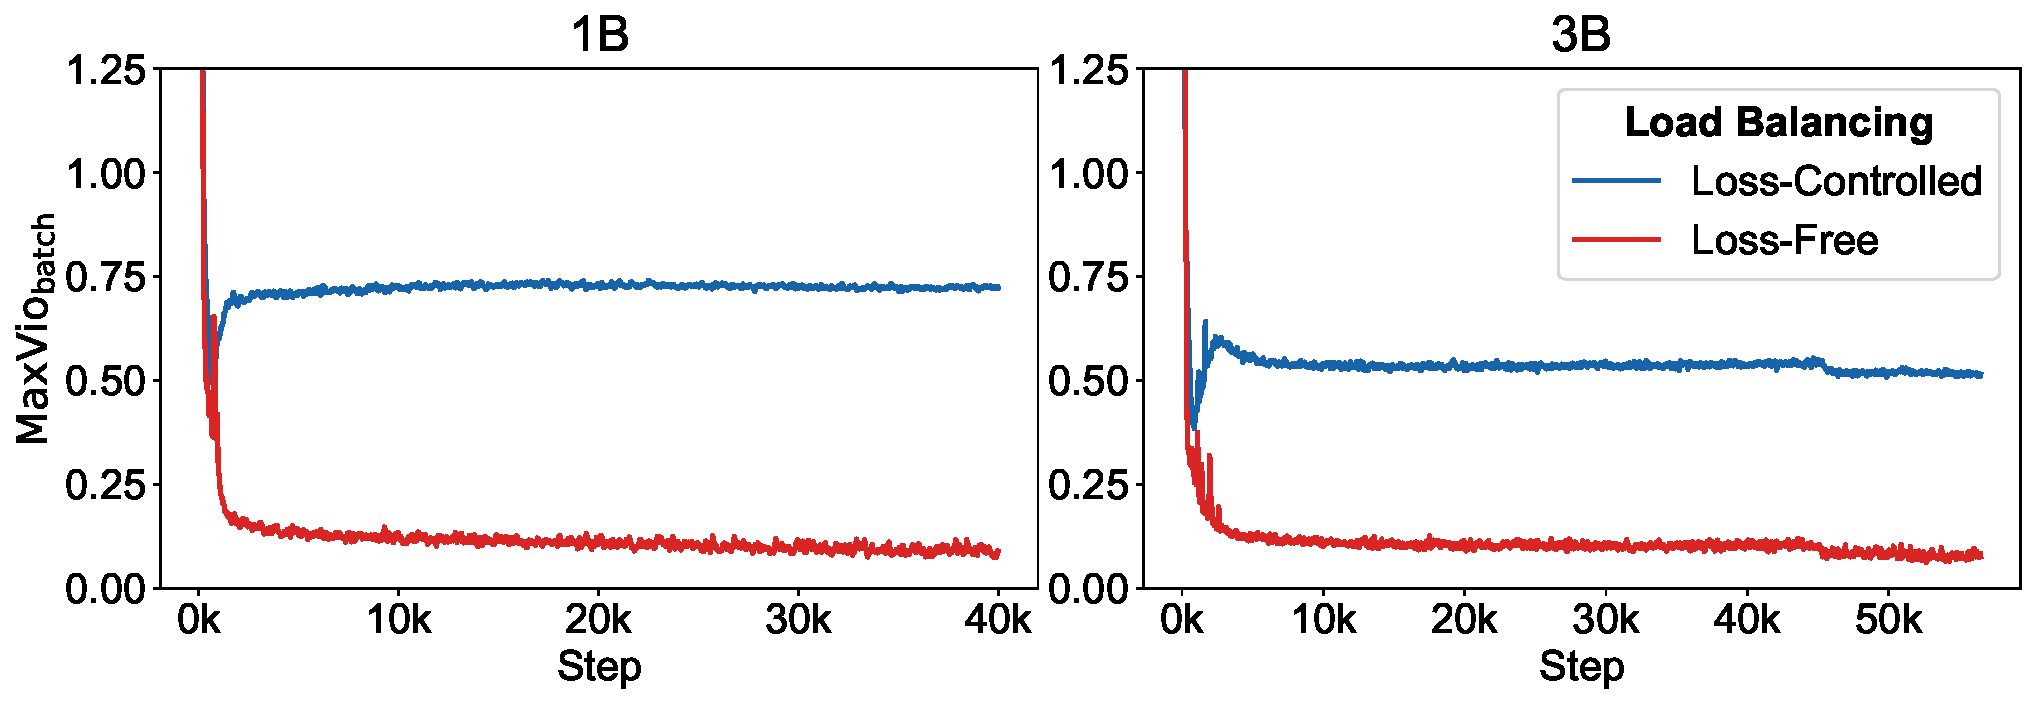
\includegraphics[width=1.0\textwidth]{figures/my_paper/update_rate_violations_main_avg100step_combined.pdf}
    \caption{训练过程中批次级负载均衡（MaxVio\textsubscript{batch}）的动态对比。}
    \label{fig:training_dynamics}
\end{figure}

\subsection{与专家并行（Expert Parallelism）的兼容性}
在训练超大规模混合专家模型时，通常会采用专家并行技术，即将不同的专家分布到不同的计算设备上。在这种设置下，计算批次（一次专家并行all-to-all涉及的数据，Computation Batch）内的负载均衡至关重要，因为它直接影响到设备间的通信开销和计算效率。

我们研究了无辅助损失均衡策略在不同计算批次大小下的表现。如图 \ref{fig:expert_parallelism_compatibility} 所示，随着计算批次大小的增加（这通常是专家并行度提高的结果），无辅助损失均衡策略的负载均衡效果会持续改善。相比之下，辅助损失方法的均衡效果在批次大小达到一定程度后便不再提升。这表明，\textbf{我们的无辅助损失均衡策略与专家并行天然兼容，并且在并行规模越大时，其优势越明显}。

\begin{figure}[h]
    \centering
    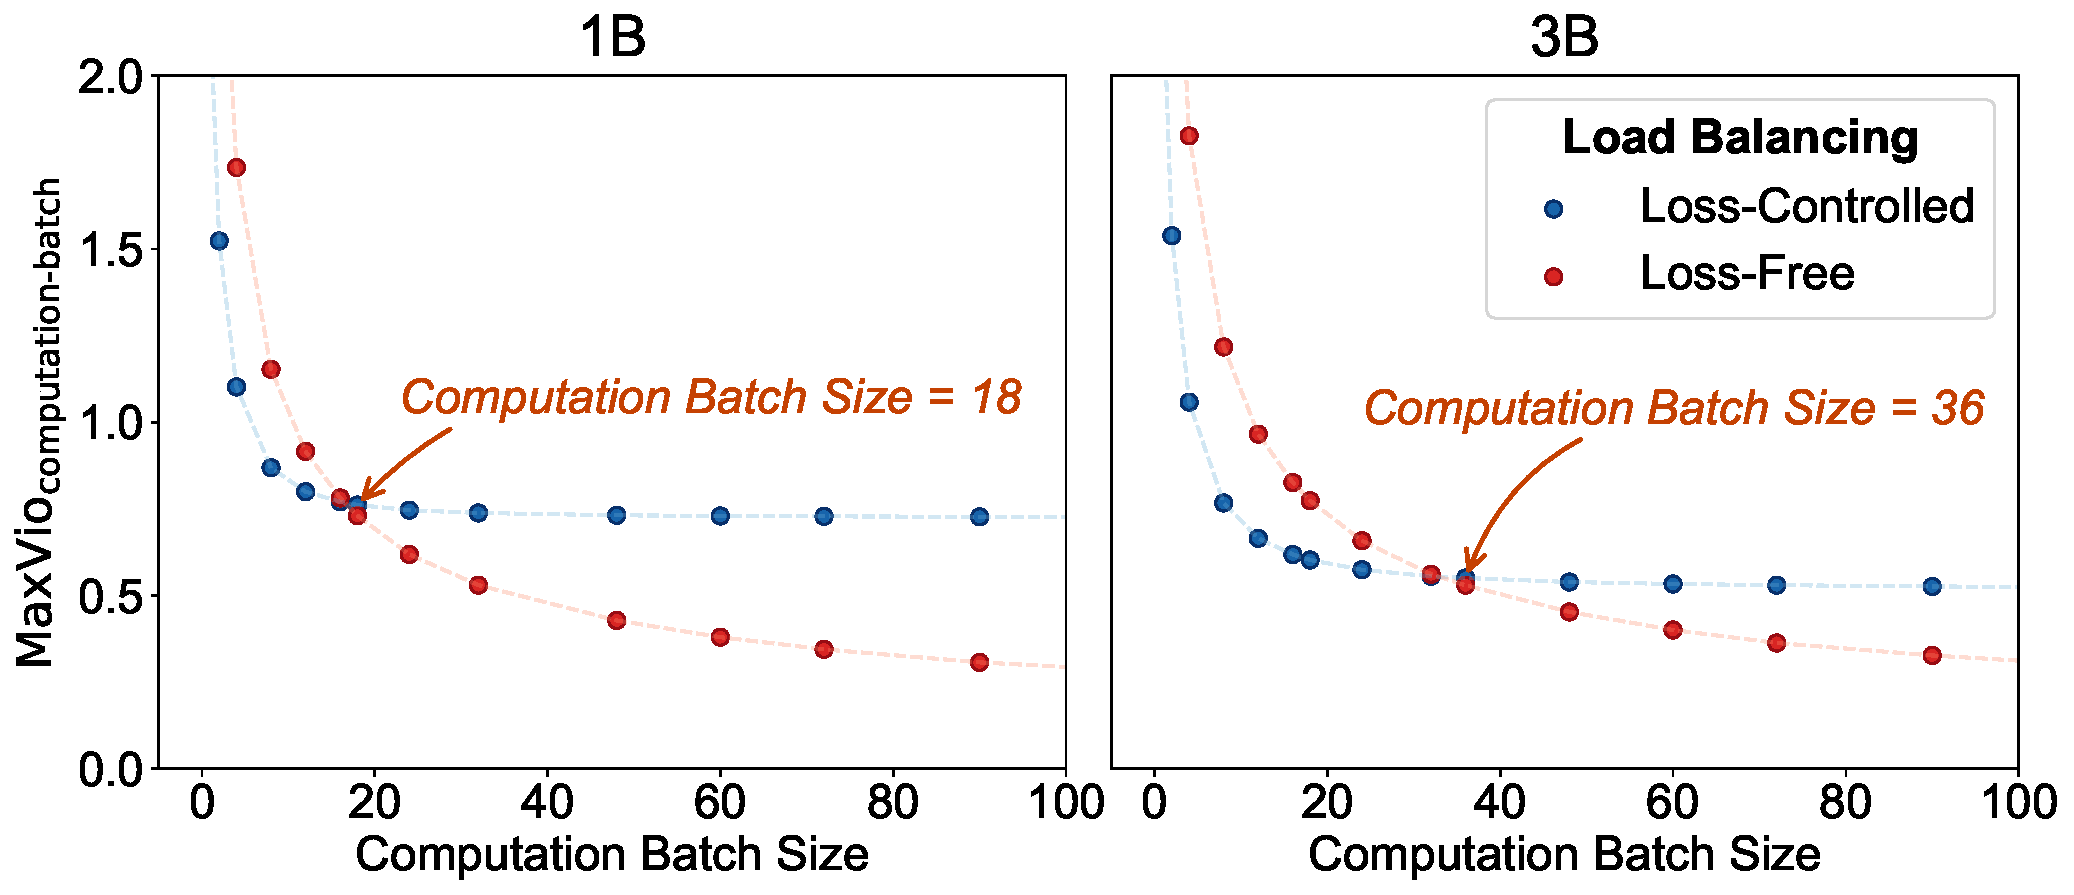
\includegraphics[width=1.0\textwidth]{figures/my_paper/actual_batch_violation_combined.pdf}
    \caption{随着计算批次大小增加，不同均衡策略的负载均衡表现。}
    \label{fig:expert_parallelism_compatibility}
\end{figure}

\subsection{与专家选择路由（Expert Choice Routing）的对比和未来词元泄露问题}
\label{sec:ec_leakage}
在负载均衡策略的探索中，除了主流的辅助损失函数方法，专家选择路由（Expert Choice Routing, EC）是另一种能够实现完美负载均衡的代表性方法\cite{Zhou2022MixtureofExpertsWE}。与传统方法中“词元选择专家”不同，专家选择路由的核心思想是“专家选择词元”：对于一个批次内的所有词元，每个专家会选择与自身亲和度最高的$k$个词元进行处理。通过设定一个全局统一的容量（capacity）$k$，可以保证每个专家处理完全相同数量的词元，从而从机制上消除了负载不均衡。

然而，专家选择路由存在一个与自回归语言模型根本原则相悖的严重问题：\textbf{未来词元泄露（Future Token Leakage）}\cite{Wang2024AuxiliaryLossFreeLB}。在标准的自回归模型训练中，模型在预测当前词元时，只能依赖于其之前的词元信息，这种因果约束（Causal Constraint）是模型泛化能力的基础。专家选择路由为了在整个词元序列（或一个计算块，chunk）中实现完美的负载均衡，其路由决策需要依赖该序列中的所有词元。这意味着，一个序列中较早位置的词元（例如$x_t$）的专家分配决策，会受到其后出现的词元（例如$x_{t+n}$）的影响（图\ref{fig:ec_leakage}）。

\begin{figure}[h]
    \centering
    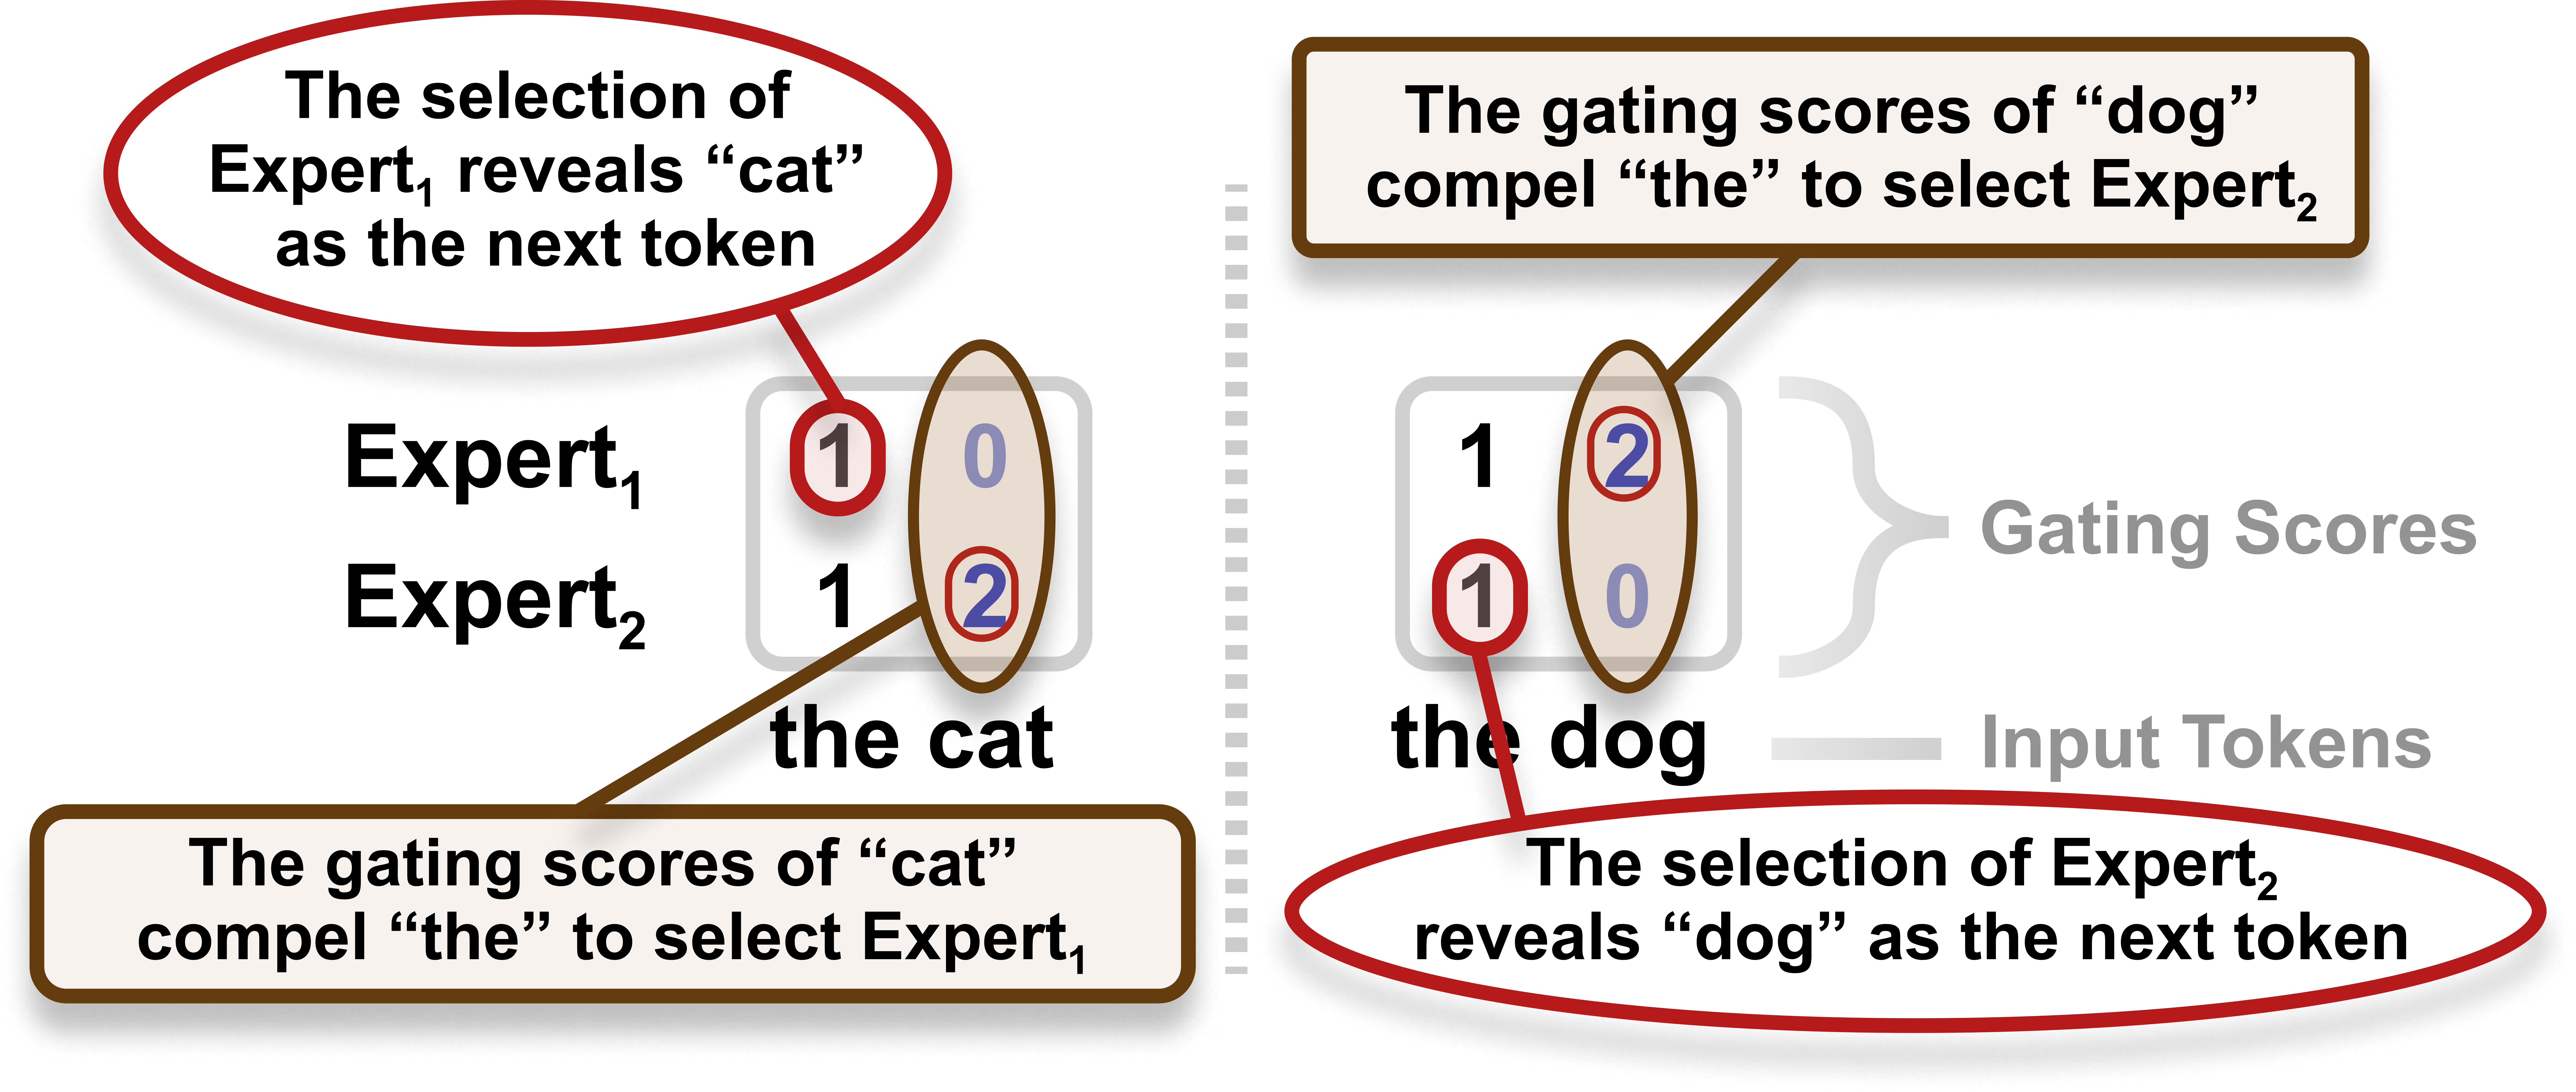
\includegraphics[width=1.0\textwidth]{figures/my_paper/EC_fig_new.png}
    \caption{后面的词元通过影响路由决策影响前面词元的混合专家模型层输出}
    \label{fig:ec_leakage}
\end{figure}

这种信息泄露是致命的，因为它使得模型在训练时可以“偷看”未来的信息来降低损失，影响了模型的正常学习，且使得训练损失失真（图\ref{fig:ec_leakage_curve}）。理论分析表明，对于一个稀疏率为$R$（即$K/N$，激活专家数除以总专家数）的混合专家模型层，EC路由每个词元最多可以泄露大约$K \log_2(\frac{1-R}{R})$比特的信息\cite{Wang2024AuxiliaryLossFreeLB}。在一个包含9个混合专家模型层、稀疏率为$1/8$（例如，从16个专家中选择2个）的典型模型中，泄露的信息总量（约50比特）足以让当前词元推断出下一个词元的身份。

\begin{figure}[h]
    \centering
    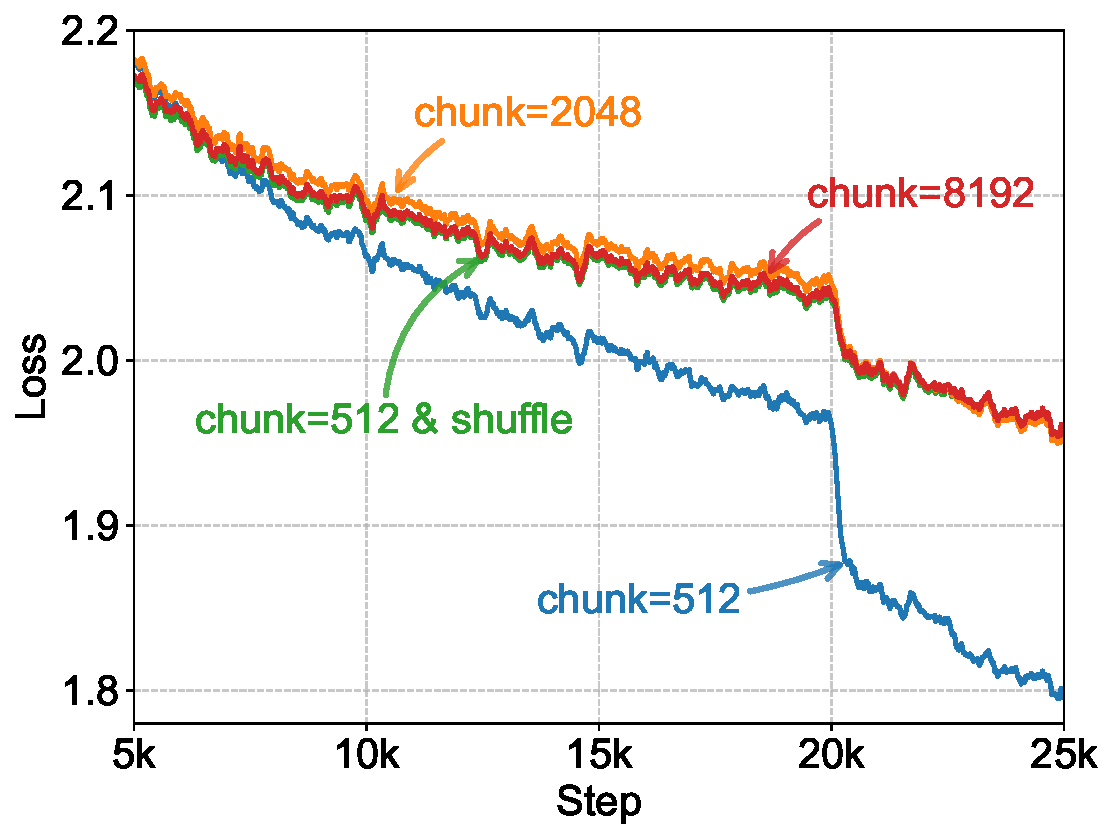
\includegraphics[width=0.7\textwidth]{figures/my_paper/ec_leakage.pdf}
    \caption{专家选择路由一次选择的范围（chunk）对训练损失的影响。范围越小，模型越容易利用信息泄露（图中蓝线），使训练损失异常降低；而打乱顺序则抑制了这种泄露（绿线）。}
    \label{fig:ec_leakage_curve}
\end{figure}

相比之下，我们提出的无辅助损失均衡策略通过基于历史批次的负载信息来更新偏置项，严格遵守了因果约束，不存在未来词元泄露的风险。这使得我们的方法在保证高效负载均衡的同时，能够更安全地应用于大规模自回归语言模型的训练。

\subsection{偏置更新算法的进一步研究}
\label{sec:bias_update_empirical}
为了验证我们在5.2.1节中提出的偏置项动态更新算法的有效性与最优配置，我们进行了一系列深入分析\cite{Wang2024AuxiliaryLossFreeLB}。研究主要围绕更新率、更新规则以及偏置形式这几个关键方面展开。

\paragraph{更新率（Update rate）的影响}
偏置项的更新率超参数$u$控制着偏置$b_i$收敛到“合适值”的速度。我们实验了不同的更新率设置，结果如图\ref{fig:update_rate_impact}所示。实验发现：
\begin{itemize}
    \item 一个过低的更新率（例如，$u=0.0001$）会导致偏置项收敛过慢。在训练初期，负载不均衡的问题得不到及时纠正。
    \item 一个过高的更新率（例如，$u=0.01$）虽然在初期能快速调整负载，但在训练后期，当负载已经趋于稳定时，过大的更新幅度反而会引入不必要的波动，破坏负载均衡的稳定性。
    \item 一个适中的更新率（例如，$u=0.001$）在收敛速度和后期稳定性之间取得了最佳平衡，能够在整个训练过程中保持良好且稳定的负载均衡效果，同时获得最优的模型性能（以困惑度衡量）。
\end{itemize}

\begin{figure}[h]
    \centering
    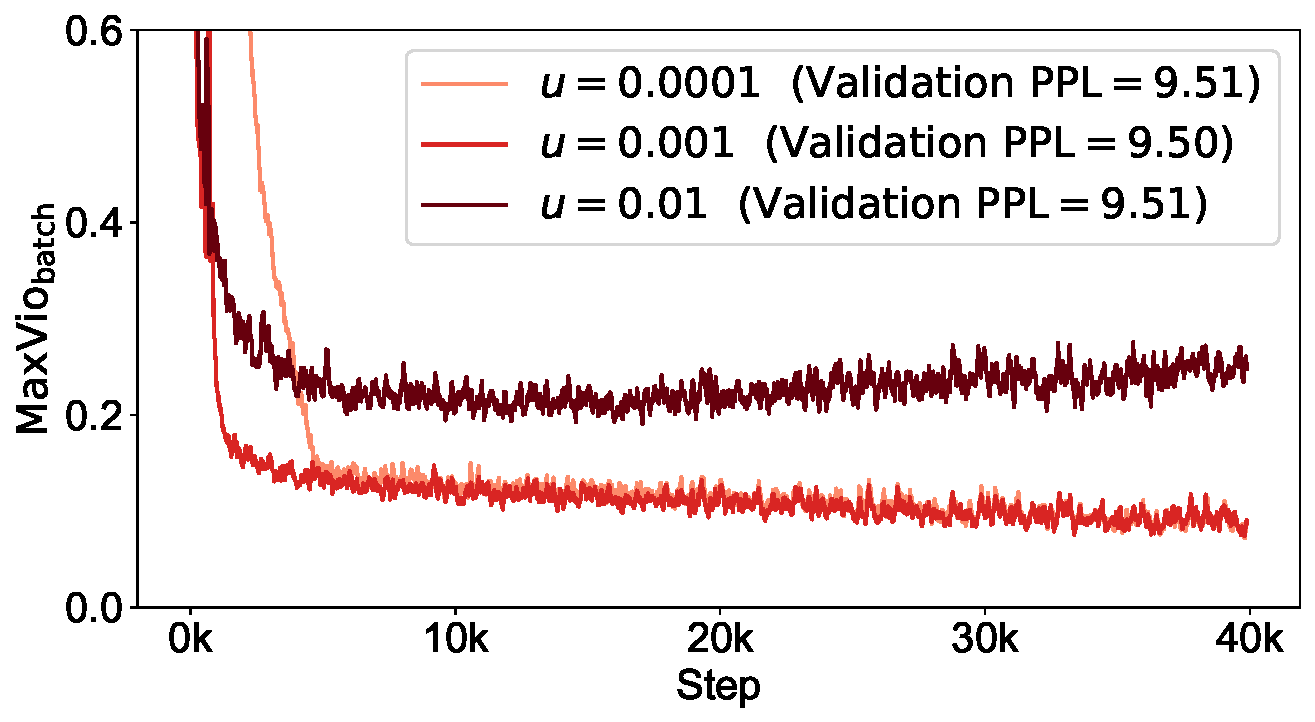
\includegraphics[width=0.7\textwidth]{figures/my_paper/update_rate_violations_avg100step.pdf}
    \caption{不同的更新率设置下，训练过程中的负载均衡}
    \label{fig:update_rate_impact}
\end{figure}

\paragraph{更新规则（Update rule）的比较}
我们使用的标准更新规则是基于负载违规误差$e_i$的符号，即 $b_i \leftarrow b_i + u \cdot \text{sign}(e_i)$。我们还研究了一种直接使用违规误差本身的变体规则：$b_i \leftarrow b_i + u \cdot e_i$。该规则旨在让负载偏差越大的专家，其偏置的调整幅度也越大。实验结果（见表\ref{tab:update_rule_comparison}）表明，尽管使用$e_i$直接更新能够在负载均衡指标上取得轻微优势，但并未带来模型最终性能的提升。考虑到符号更新规则的简洁性和鲁棒性，我们最终选择其作为标准算法。

\begin{table}[t]
\caption{不同更新规则的对比}
\label{tab:update_rule_comparison}
\begin{center}
\begin{tabular}{l|c|c}
\toprule
\multicolumn{1}{c|}{\textbf{Method}} & \textbf{Perplexity} & $\textbf{MaxVio}_\textbf{global}$ \\
\midrule
$b_i =  b_i + u*\text{sign}(e_i)$, $u=0.001$ & \textbf{9.50} & 0.044 \\
$b_i = b_i + u*e_i$, $u=0.01$ & 9.53 & \textbf{0.028}\\ 
$ b_i =  b_i + u*e_i$, $u=0.001$ &  9.51 & 0.036 \\
$ b_i = b_i + u*e_i$, $u=0.0001$ & 9.51  & 0.040 \\
\bottomrule
\end{tabular}
\end{center}
\end{table}

\paragraph{乘性偏置（Multiplicative bias）的可行性}
除了在我们路由分数上引入加性偏置（additive bias），我们还探索了使用乘性偏置（multiplicative bias）的可能性。即，路由决策由$\text{TopK}(\{s_{j,t} \cdot b_j|1\leq j\leq N\},K)$决定，其中偏置项$b_i$初始化为1。更新逻辑与加性偏置类似。实验对比（见表\ref{tab:multiplicative_bias_comparison}）发现，使用乘性偏置在负载均衡效果上与加性偏置相近，但会导致模型性能轻微下降。因此，我们最终确定加性偏置是更优越的选择。

\begin{table}[t]
\caption{加性偏置与乘性偏置的对比}
\label{tab:multiplicative_bias_comparison}
\begin{center}
\begin{tabular}{l|c|c}
\toprule
\multicolumn{1}{c|}{\textbf{Method}} & \textbf{Perplexity} & $\textbf{MaxVio}_\textbf{global}$ \\
\midrule
Addative Bias, $u=0.001$ & \textbf{9.50} & 0.044 \\
Multiplicative Bias, $u=0.01$ & 9.52 & 0.041 \\ 
Multiplicative Bias, $u=0.001$ &  9.52 & \textbf{0.036} \\
Multiplicative Bias, $u=0.0001$ & 9.54  & 0.048 \\
\bottomrule
\end{tabular}
\end{center}
\end{table}

\section{无辅助损失均衡策略的应用}
无辅助损失均衡策略作为一种简单、灵活、有效的混合专家模型负载均衡调控方法，已经在工业界得到了广泛应用。最近一年发布的国产开源大语言模型DeepSeek-V3~\cite{DeepSeekAI2024DeepSeekV3TR}，Kimi K2~\cite{Bai2025KimiKO}和GLM-4.5\cite{Zeng2025GLM45AR}均使用了这一方法。特别的，对于传统Top-K之外的场景，如不同专家计算量不同的情况，无辅助损失均衡策略也能高效的调控各个专家的负载乃至词元分配到的平均计算量。Grove MoE\cite{Wu2025GroveMT}使用它控制引入伴随专家情况下的负载均衡，而最近发布的大模型LongCat-Flash\cite{meituan-longcat_2025_longcat-flash-chat}也使用了这一策略来控制带零计算专家情况下的负载均衡。

\section{本章小结}
\label{sec:chapter_summary_personal}
本章详细介绍了我们在混合专家模型负载均衡方向的个人研究进展——一种无需辅助损失的无辅助损失均衡策略（Auxiliary-Loss-Free Balancing）。该策略通过引入并动态更新一个专家级的偏置项，直接在路由选择阶段主动引导负载均衡，从而避免了传统辅助损失方法所带来的“性能-均衡”困境。

我们的主要贡献包括：
\begin{enumerate}
    \item \textbf{提出了一个新的负载均衡框架}：该框架不依赖于损失函数和梯度，从根本上消除了对主任务训练的干扰。
    \item \textbf{设计了简洁有效的算法}：通过简单的偏置更新规则，实现了强大而稳定的负载控制。
    \item \textbf{进行了充分的实验验证}：在不同规模的模型上证明了该策略相比传统方法，在模型性能和负载均衡两方面均取得显著优势。
    \item \textbf{分析了其优势和兼容性}：阐明了其在避免信息泄露和与大规模并行训练兼容性方面的优点。
\end{enumerate}

这项研究为解决混合专家模型训练中的一个核心挑战提供了新的思路和有效的工具，对大规模、高效的稀疏模型研发具有重要的实践意义。